\section{Simulation}\label{sec:sim}

	\begin{figure}		
		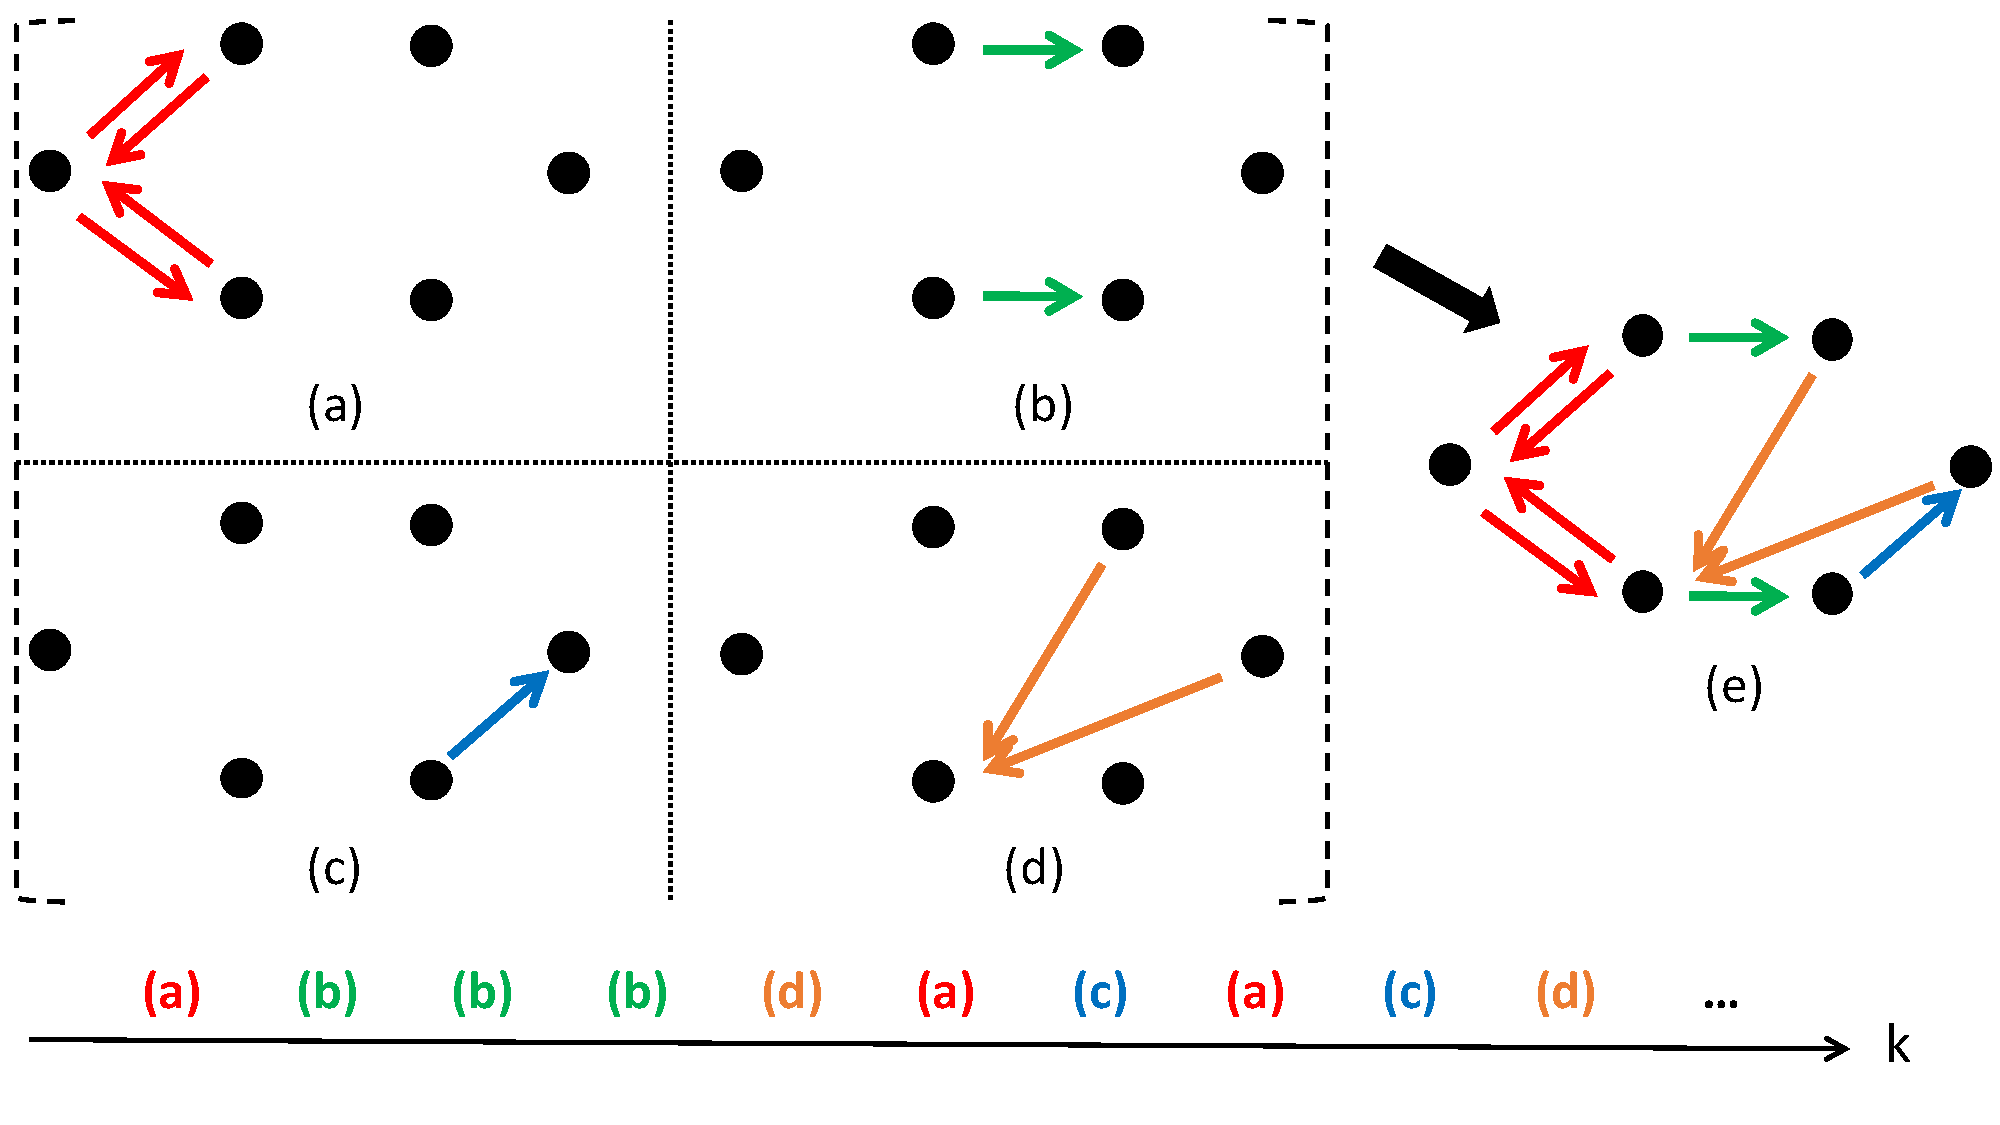
\includegraphics[width=0.5\textwidth]{figures/switch_topo}
		\caption{The dynamically changing topologies used in the simulation: (a)-(d) four types of topologies; (e) the union of these topologies is jointly strongly connected; (f) a randomly generated sequence of topologies that satisfy the \fc ness condition.}\label{fig:com_topo}		
	\end{figure}
	
	\begin{figure}%[thpb]
		\centering		
		\begin{subfigure}[b]{0.23\textwidth}
			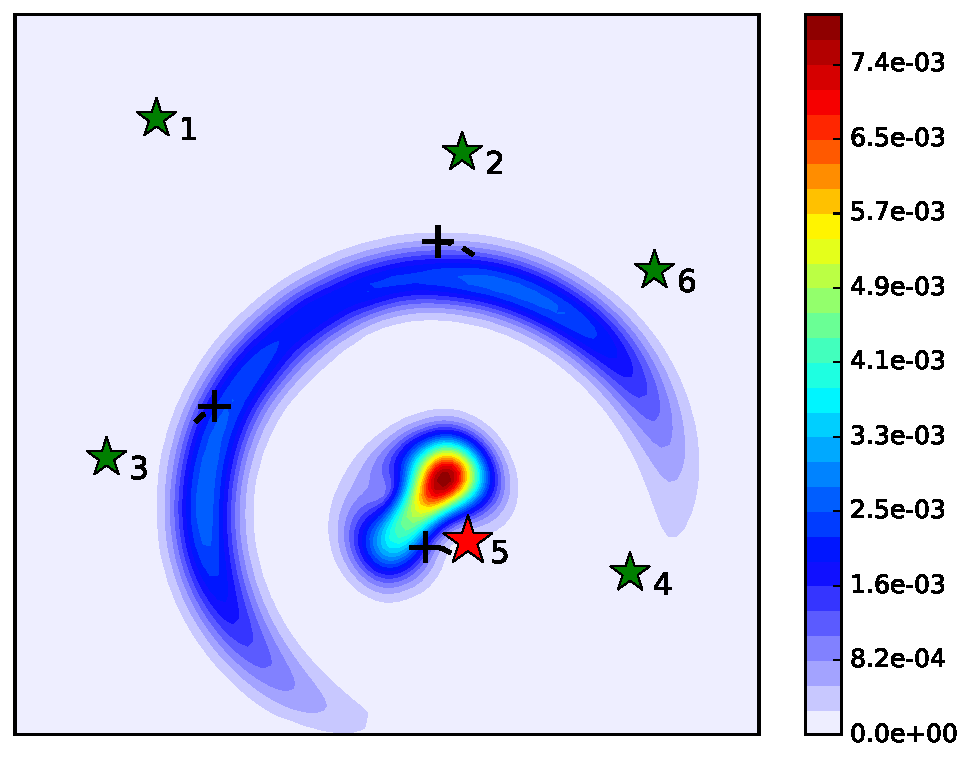
\includegraphics[width=\textwidth]{figures/dbf_hetero_mov_sen_mov_tar_rbt5_step3}
			\caption{\proto-DBF Step 3}\label{fig:step3}
		\end{subfigure}
		\begin{subfigure}[b]{0.23\textwidth}
			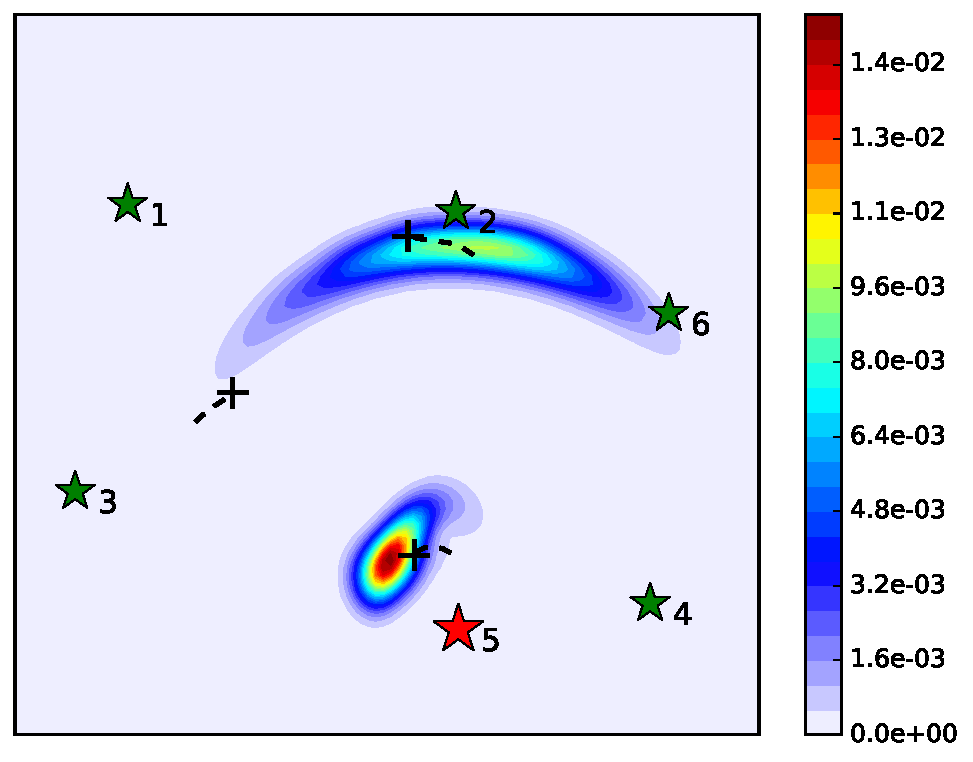
\includegraphics[width=\textwidth]{figures/dbf_hetero_mov_sen_mov_tar_rbt5_step5}
			\caption{\proto-DBF at Step 5}\label{fig:step5}
		\end{subfigure}
		\begin{subfigure}[b]{0.23\textwidth}
			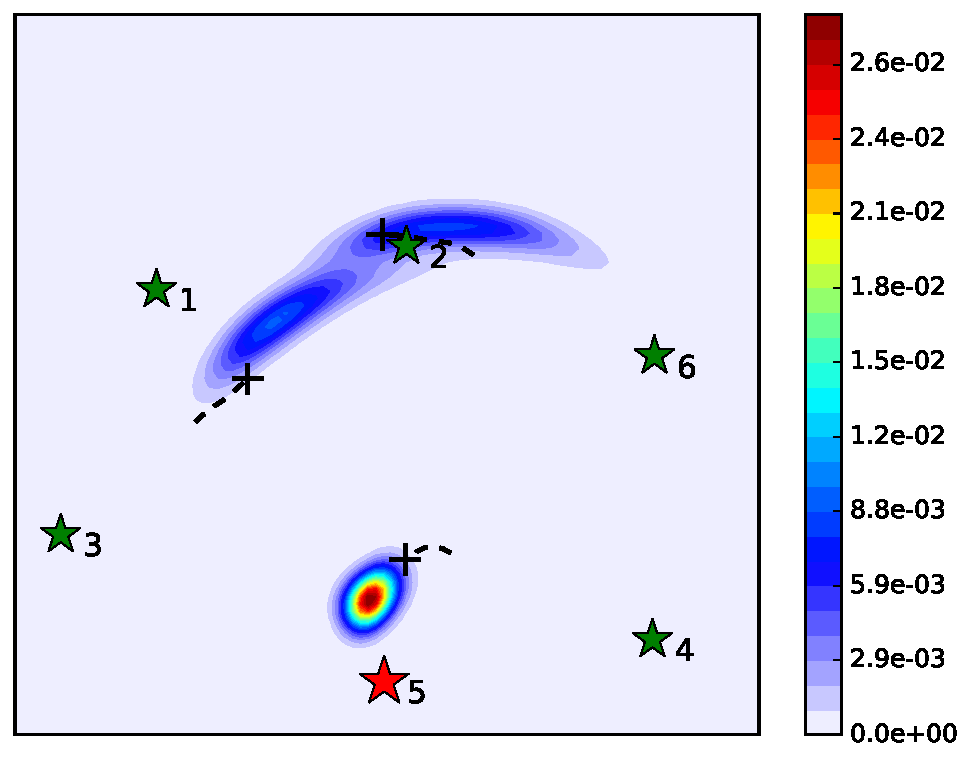
\includegraphics[width=\textwidth]{figures/dbf_hetero_mov_sen_mov_tar_rbt5_step7}
			\caption{\proto-DBF at Step 7}\label{fig:step7}
		\end{subfigure}
		\begin{subfigure}[b]{0.23\textwidth}
			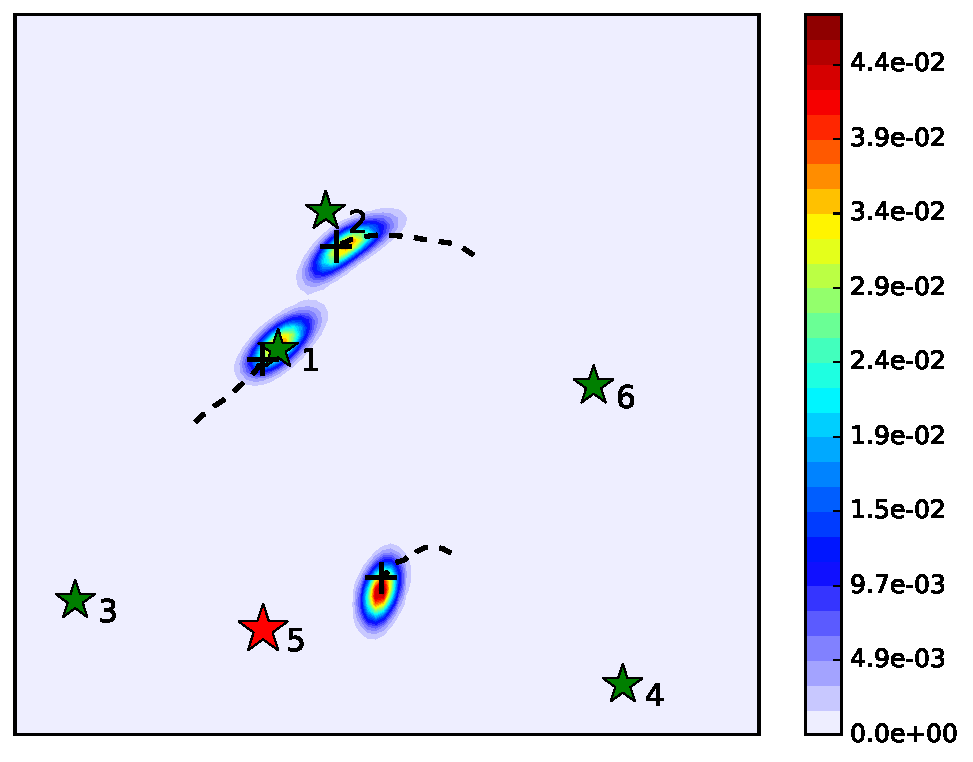
\includegraphics[width=\textwidth]{figures/dbf_hetero_mov_sen_mov_tar_rbt5_step10}
			\caption{\proto-DBF at Step 10}\label{fig:step10}
		\end{subfigure}
		\begin{subfigure}[b]{0.23\textwidth}
			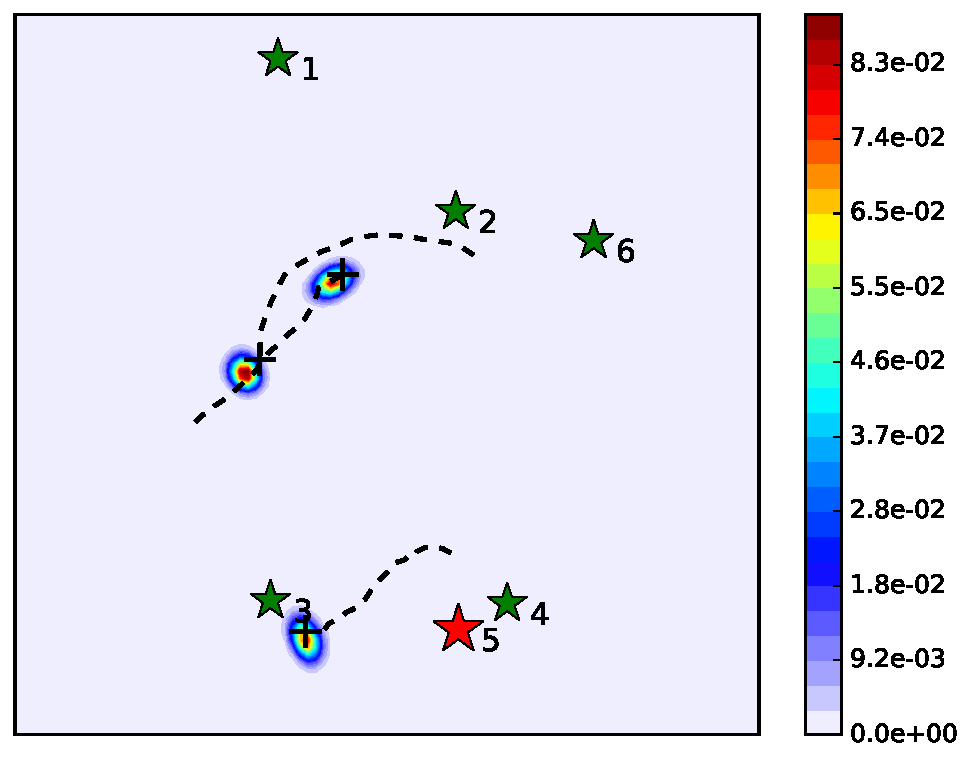
\includegraphics[width=\textwidth]{figures/dbf_hetero_mov_sen_mov_tar_rbt5_step20}
			\caption{\proto-DBF at Step 20}\label{fig:step20}
		\end{subfigure}	
		\begin{subfigure}[b]{0.23\textwidth}
			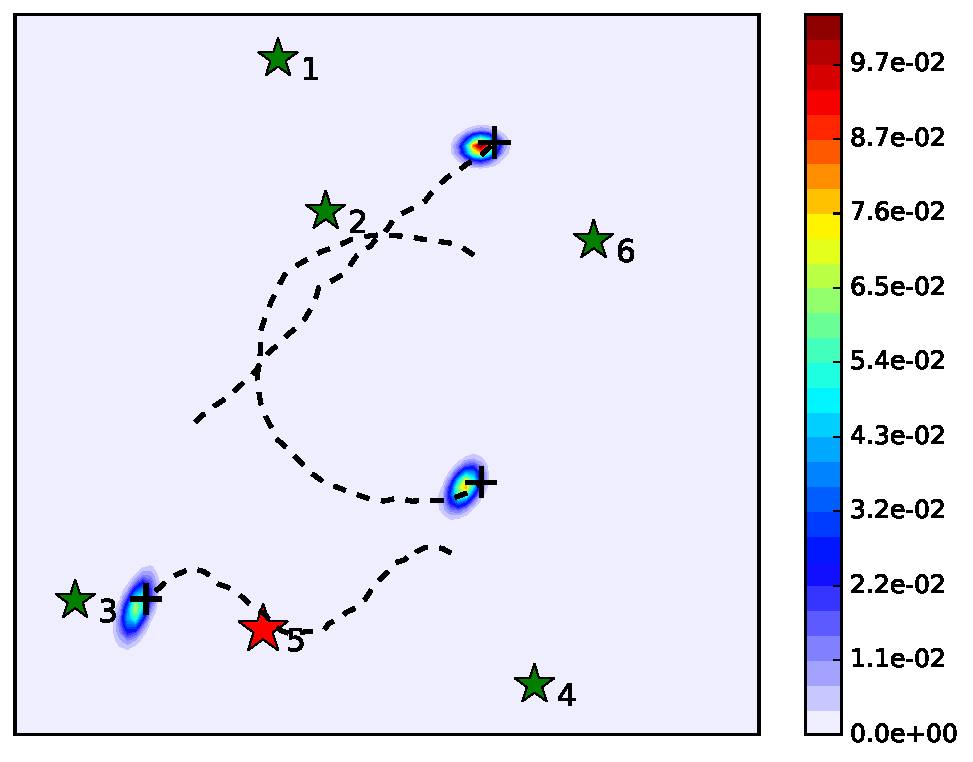
\includegraphics[width=\textwidth]{figures/dbf_hetero_mov_sen_mov_tar_rbt5_step40}
			\caption{\proto-DBF at Step 40}\label{fig:step40}
		\end{subfigure}	
		\begin{subfigure}[b]{0.23\textwidth}
			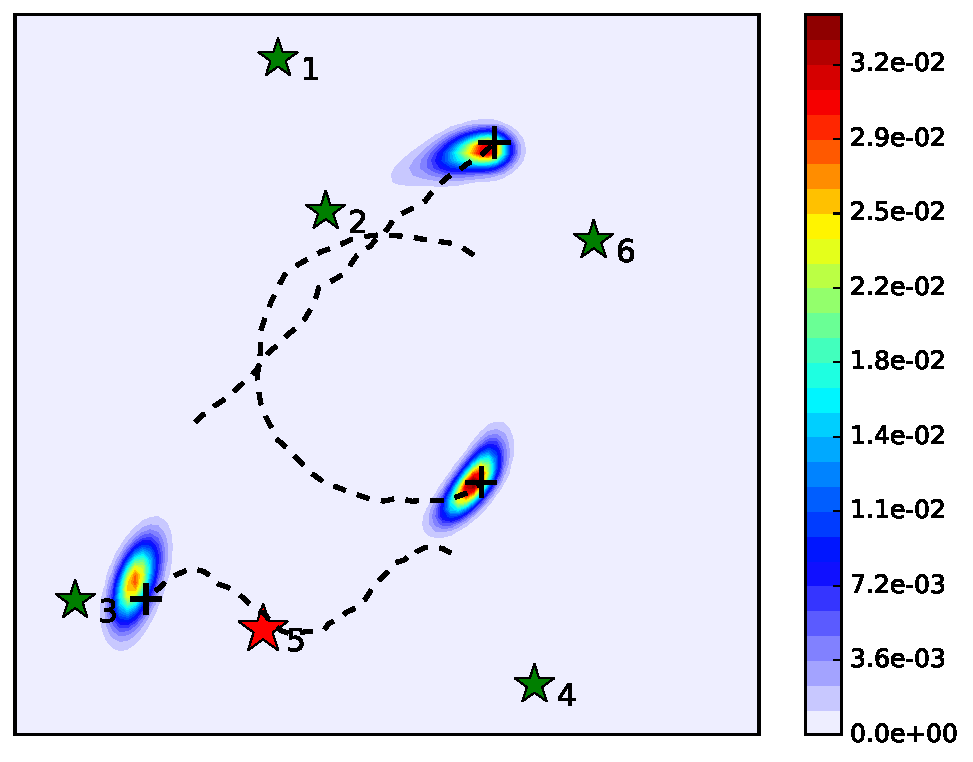
\includegraphics[width=\textwidth]{figures/cons_hetero_mov_sen_mov_tar_rbt5_step40}
			\caption{CbDF at Step 40}\label{fig:cbdf_step40}
		\end{subfigure}	
		\begin{subfigure}[b]{0.23\textwidth}
			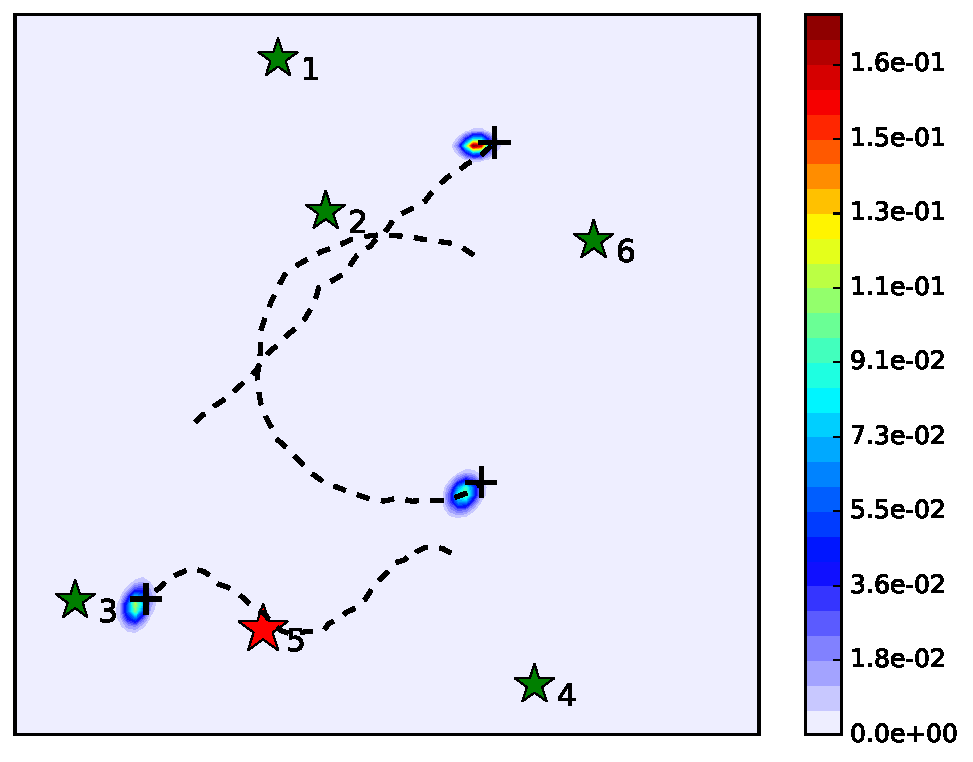
\includegraphics[width=\textwidth]{figures/cent_hetero_mov_sen_mov_tar_rbt1_step40}
			\caption{CF at Step 40}\label{fig:cf_step40}
		\end{subfigure}
		\caption{First scenario: (a) two types of topologies; (b) individual PDF of the $3^\text{rd}$ UGV after initial observation; (c)-(e) PDFs at the end of simulation using different filters; (f) average position estimation errors; (g) average entropy of PDF. In last two figures, metrics are based on the PDFs of the $1^\text{st}$, $3^\text{rd}$ and $5\thi$ UGV using \proto-DBF, the common PDF using CbDF and using CF.}
		\label{fig:mov_sen_mov_tar1}
		%		\vspace{-1.3em}
	\end{figure}
	
	We conduct a simulation that uses a team of six UGVs to localize three moving targets.
	Every UGV maintains three individual PDFs, each corresponding to a target.
	At each time step, a UGV's sensor can measurement the positions of three targets.
	We assume that the UGVs know the association between the measurement and the corresponding target.
	The targets have different motion models, including the linear motion (target $1$), sinusoidal motion (target $2$), and circular motion (target $3$).
	Three of the UGVs have range-only sensors and the other three UGVs have bearing-only sensors.
	The interaction topology of the UGVs is time-varying and consists of four types, as shown in \cref{fig:com_topo}(a)-(d).
	A randomly generated sequence of topologies is used (\cref{fig:com_topo}f).
	It can be noticed that, the interaction topology is \fc when all four types appears repeatedly (\cref{fig:com_topo}e).
	Ten layouts of the initial positions of UGVs and targets are randomly generated.
	We compare \proto-DBF with CbDF and CF.
	
	\cref{fig:mov_sen_mov_tar1} show the simulation results of a specific layout.
	The sum of the $1^\text{st}$ UGV's individual PDFs are shown in the figures.
	\cref{fig:step3,fig:step5,fig:step7,fig:step10,fig:step20,fig:step40} show that the \proto-DBF can successfully localize and track moving target's positions and effectively reduce the estimation uncertainty, which is similar to the performance of the CF (\cref{fig:cf_step40}).
	On the contrary, CbDF is less effective to reduce the estimation uncertainty (\cref{fig:cbdf_step40}).
	
	We compares the three filters in terms of the estimation error and entropy of the uncertainty.
	The estimation error is defined as the difference between the true target position and the MAP estimate of the individual PDF:
	\small\begin{equation*}
		\Delta_k = \|x^\text{MAP}_k-x^g_k\|_2.
	\end{equation*}\normalsize
	The entropy of the uncertainty is
	\small\begin{equation*}
		H_k = \sum\limits_{X_k\in S} -P_{pdf}(X_k)\log(P_{pdf}(X_k)).
	\end{equation*}\normalsize
	The average of the estimation error and entropy of each target across ten layouts are shown in \cref{fig:metrics}.
%	For \proto-DBF, we only show the results of the $1^\text{st}$, $3^\text{rd}$, and $5\thi$ UGV for the clarity of the plots.
	It can be noticed that, the CF achieves the most accurate position estimation and fastest entropy reduction. 
	This is an expected result since the CF utilizes all sensor measurements.
	The \proto-DBF achieves similar results as the CF asymptotically. 
	This is a very interesting results, since \proto-DBF only communicates with neighboring UGVs and have a subset of other UGVs' measurements.
	The CbDF achieves similar position estimation performance and the CF and \proto-DBF. 
	However, it fails to effectively reduce the estimation entropy.
	This is because that, the linear combination of PDFs used in the CbDF does not follow the nonlinear nature of Bayesian filtering, thus information is loss during the combination.
	The \proto-DBF, on the other hand, rigorously follows the procedure of Bayesian filtering, and therefore achieves better performance.
	
	
	\begin{figure}%[thpb]
		\centering
		\begin{subfigure}[b]{0.23\textwidth}
			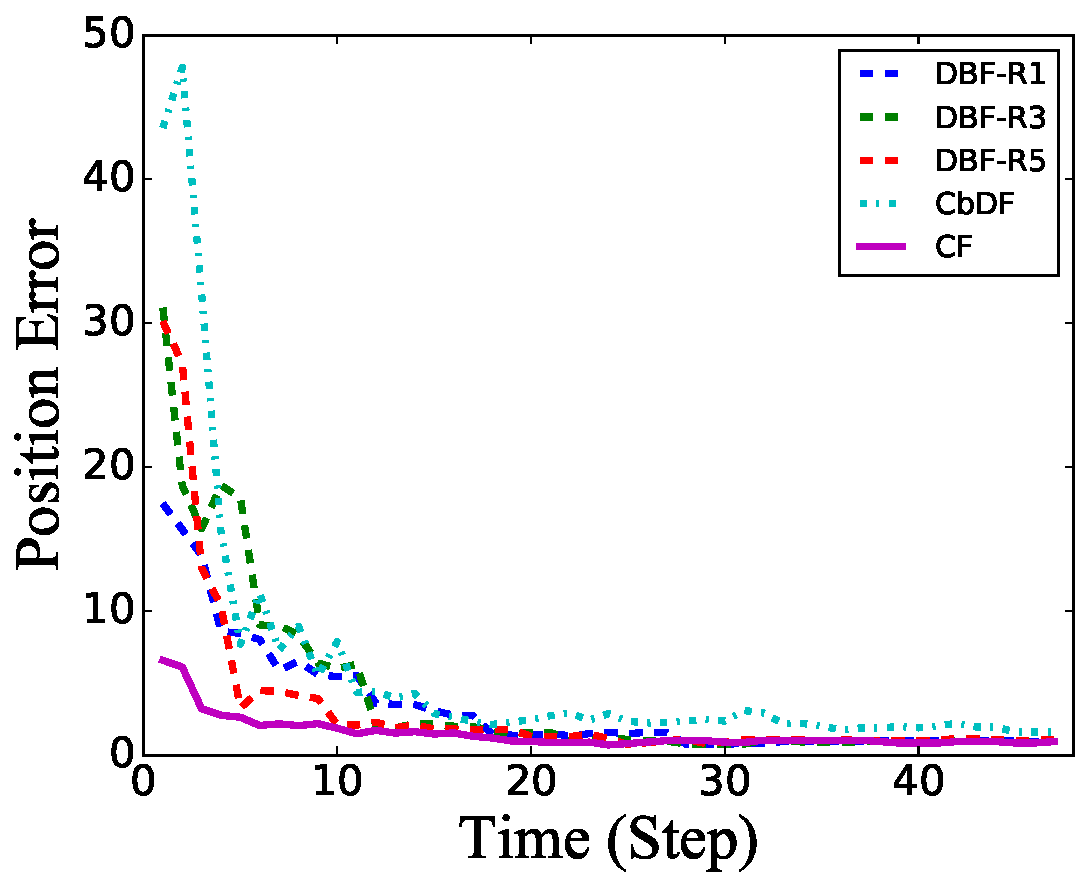
\includegraphics[width=\textwidth]{figures/hetero_mov_sen_mov_tar_pos_err_noise_linear}
			\caption{Position Error of Target $1$}\label{fig:lin_pos_err}
		\end{subfigure}				
		\begin{subfigure}[b]{0.23\textwidth}
			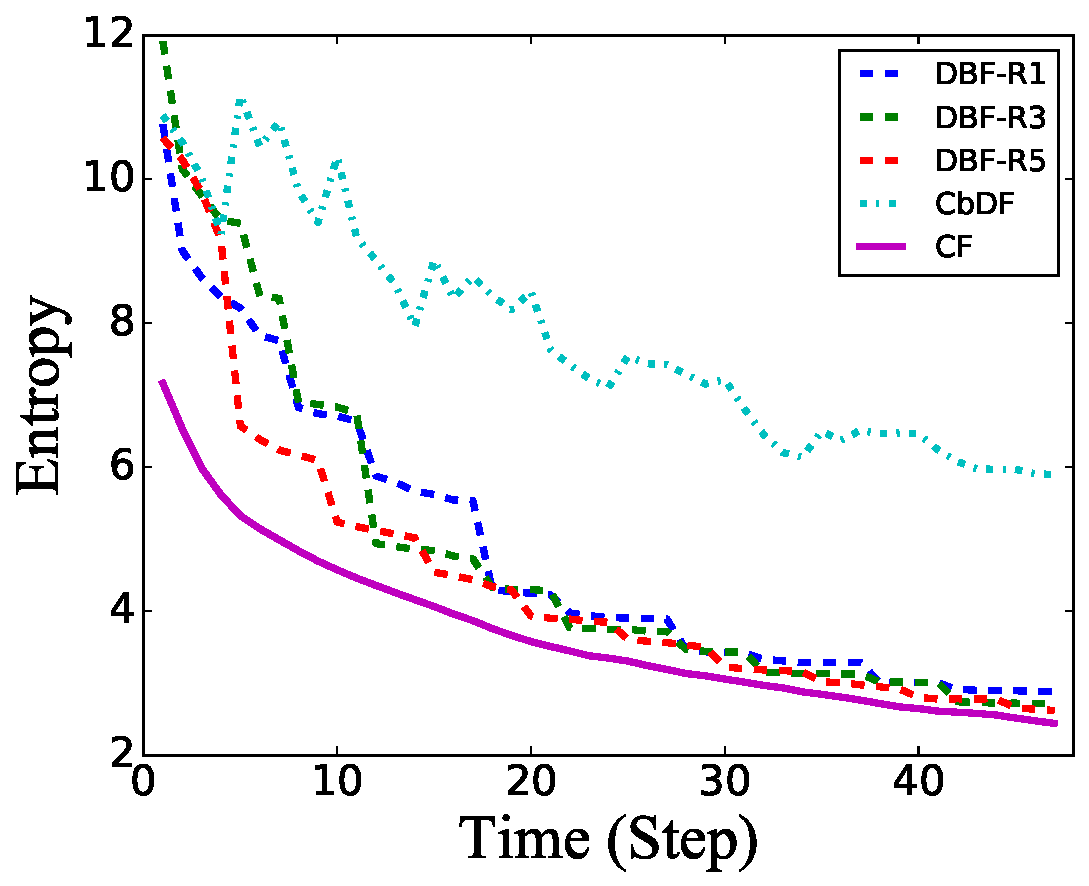
\includegraphics[width=\textwidth]{figures/hetero_mov_sen_mov_tar_entropy_noise_linear}
			\caption{Entropy of Target $1$}\label{fig:lin_ent}
		\end{subfigure}	
		\begin{subfigure}[b]{0.23\textwidth}
			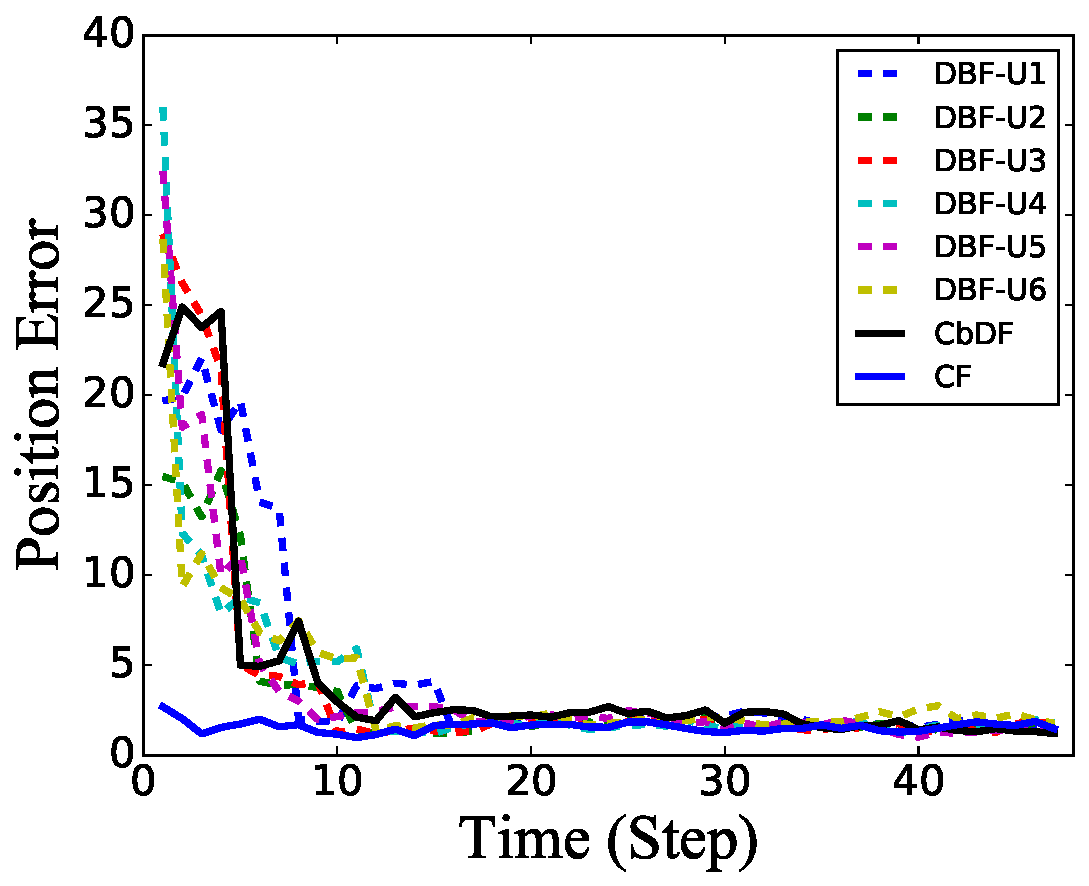
\includegraphics[width=\textwidth]{figures/hetero_mov_sen_mov_tar_pos_err_noise_circle}
			\caption{Position Error of Target $2$}\label{fig:cir_pos_err}
		\end{subfigure}
		\begin{subfigure}[b]{0.23\textwidth}
			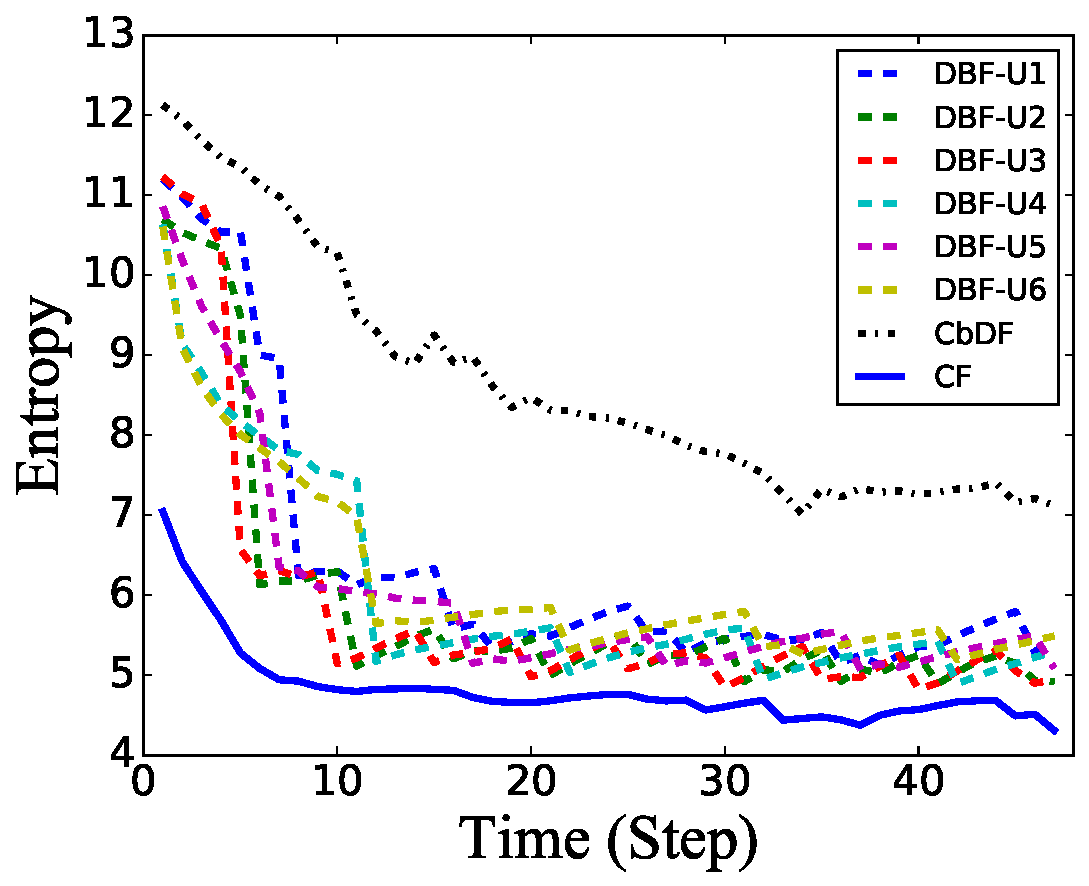
\includegraphics[width=\textwidth]{figures/hetero_mov_sen_mov_tar_entropy_noise_circle}
			\caption{Entropy of Target $2$}\label{fig:cir_ent}
		\end{subfigure}			
		\begin{subfigure}[b]{0.23\textwidth}
			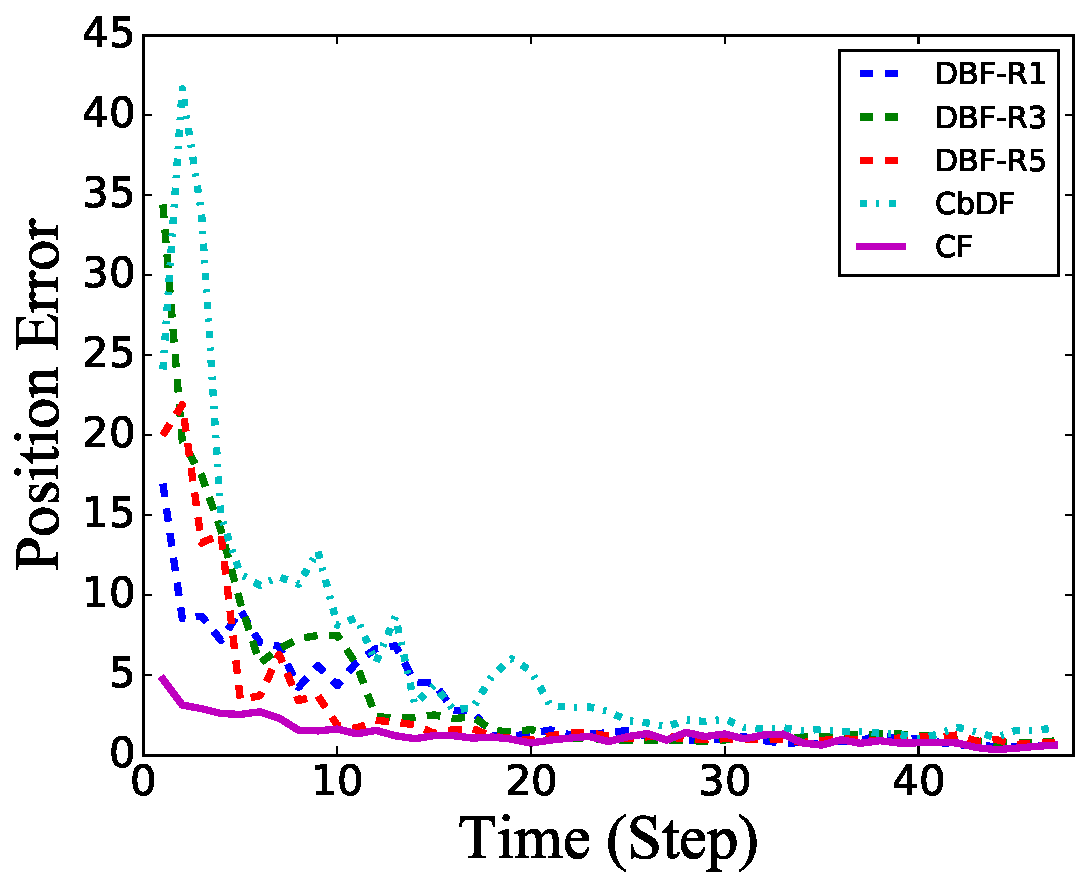
\includegraphics[width=\textwidth]{figures/hetero_mov_sen_mov_tar_pos_err_noise_sin}
			\caption{Position Error of Target $3$}\label{fig:sin_pos_err}
		\end{subfigure}
		\begin{subfigure}[b]{0.23\textwidth}
			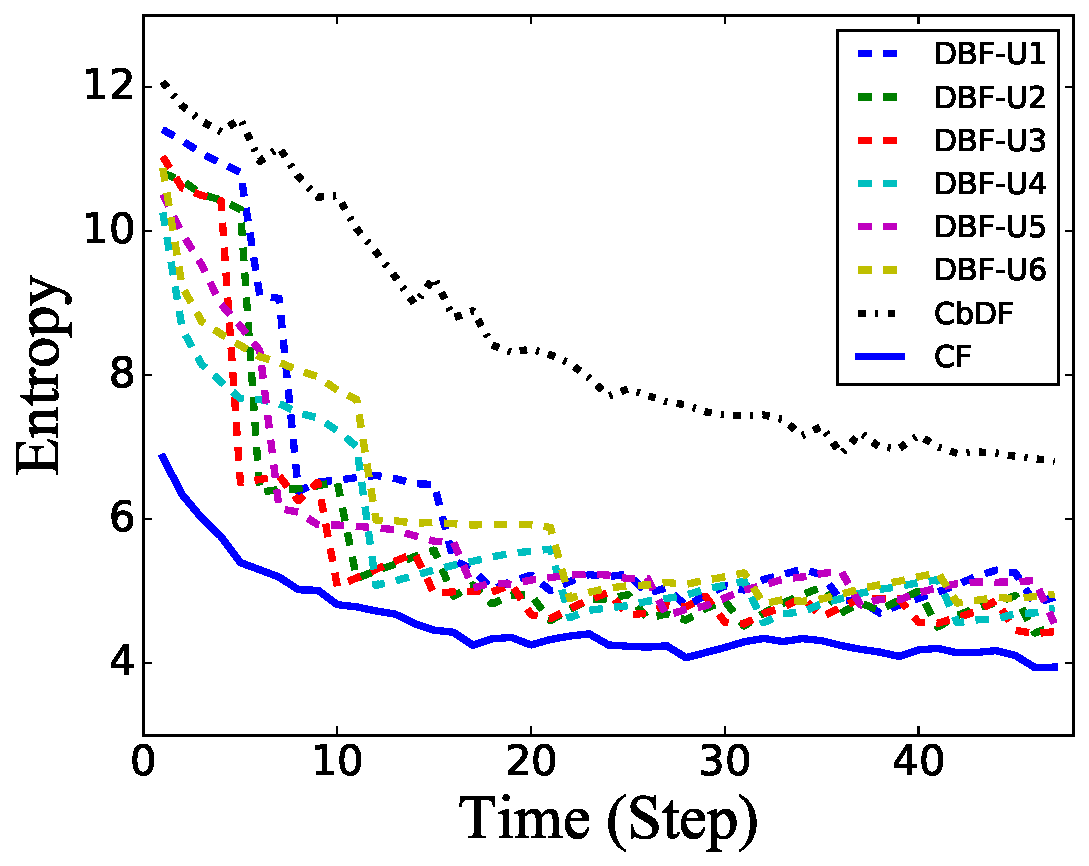
\includegraphics[width=\textwidth]{figures/hetero_mov_sen_mov_tar_entropy_noise_sin}
			\caption{Entropy of Target $3$}\label{fig:sin_ent}
		\end{subfigure}		
		\caption{First scenario: (a) two types of topologies; (b) individual PDF of the $3^\text{rd}$ UGV after initial observation; (c)-(e) PDFs at the end of simulation using different filters; (f) average position estimation errors; (g) average entropy of PDF. In last two figures, metrics are based on the PDFs of the $1^\text{st}$, $3^\text{rd}$ and $5\thi$ UGV using \proto-DBF, the common PDF using CbDF and using CF.}
		\label{fig:metrics}
		%		\vspace{-1.3em}
	\end{figure}		